\documentclass{article}
\usepackage[T1]{fontenc}
\usepackage{lmodern}
\usepackage{graphicx}
\usepackage{amsmath,amssymb}
\usepackage[a4paper,margin=2cm]{geometry}
\usepackage[absolute,overlay]{textpos}
\setlength{\TPHorizModule}{1mm}
\setlength{\TPVertModule}{1mm}
\usepackage[indonesian]{babel}
\usepackage{hyperref}
\setlength{\emergencystretch}{2em}
% unit: Halaman 71

\begin{document}

% === Halaman 71 (llm) ===

\begin{verbatim}
% Konversi biner ke desimal
L = 0;
for idx = 1:30
    L = L + double(nL(idx))*(2^(30-idx));
end

\vspace{119.39mm}

% Ekstraksi bit-bit pesan ke dalam vektor biner, bit-bit panjang pesan
% ikut dibaca kembali dari awal
m = L*8 + 30; % panjang bit pesan yang harus dibaca
disp('Ekstraksi pesan....');
idx = 1;
for row = 1 : size(stegoImage,1)
    for col = 1 : size(stegoImage,2)
        for i = 1 : 3
            if idx <= m
                vektorBiner(idx) = bitget(stegoImage(row,col, i), 1);
                idx = idx + 1;
            end
        end
    end
end
\end{verbatim}

% deskripsi: Screenshot potongan kode program MATLAB untuk konversi biner ke desimal dan ekstraksi pesan dari stegoImage.
% bbox normalisasi: [0.0600, 0.4200, 0.7830, 0.8220]
\begin{textblock*}{151.83mm}(12.60mm,124.74mm)
\noindent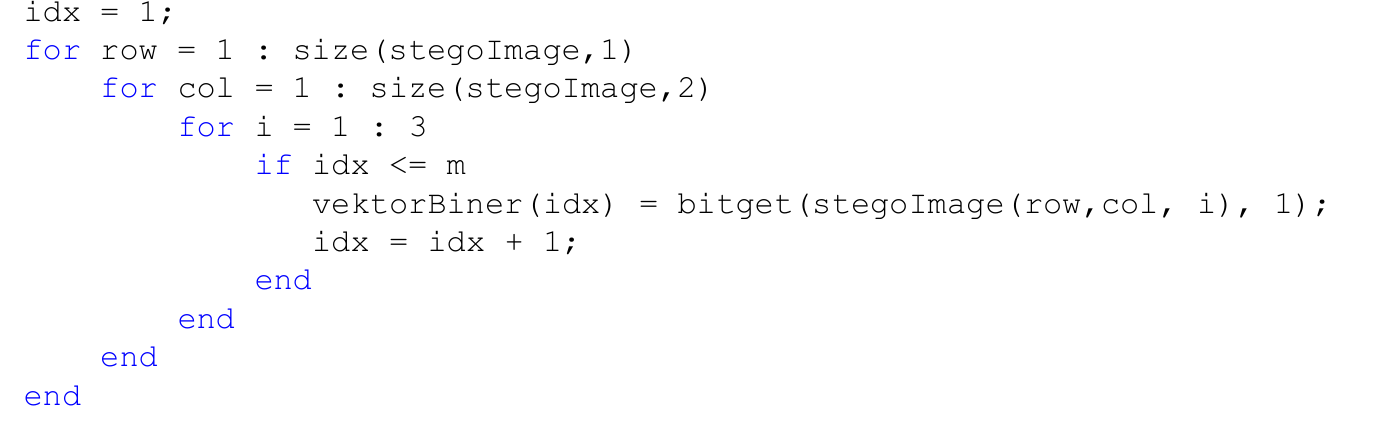
\includegraphics[width=151.83mm,height=119.39mm]{../../images/llm/page_071_img_01.png}%
\end{textblock*}

\end{document}
